% BOTTOM caption
% ------------------------
\begin{figure}[!htbp]
\centering
\vspace{1\baselineskip}
% ------------------------
%
% SIDE caption
% ------------------------
%\begin{SCfigure}[\sidecaptionrelwidth][!htbp]
%\centering
%\vspace{1\baselineskip}
%\includegraphics[width=0.5\textwidth]
% ------------------------
%
% Main information
% ===========================================================
\begin{subfigure}{0.495\textwidth}
	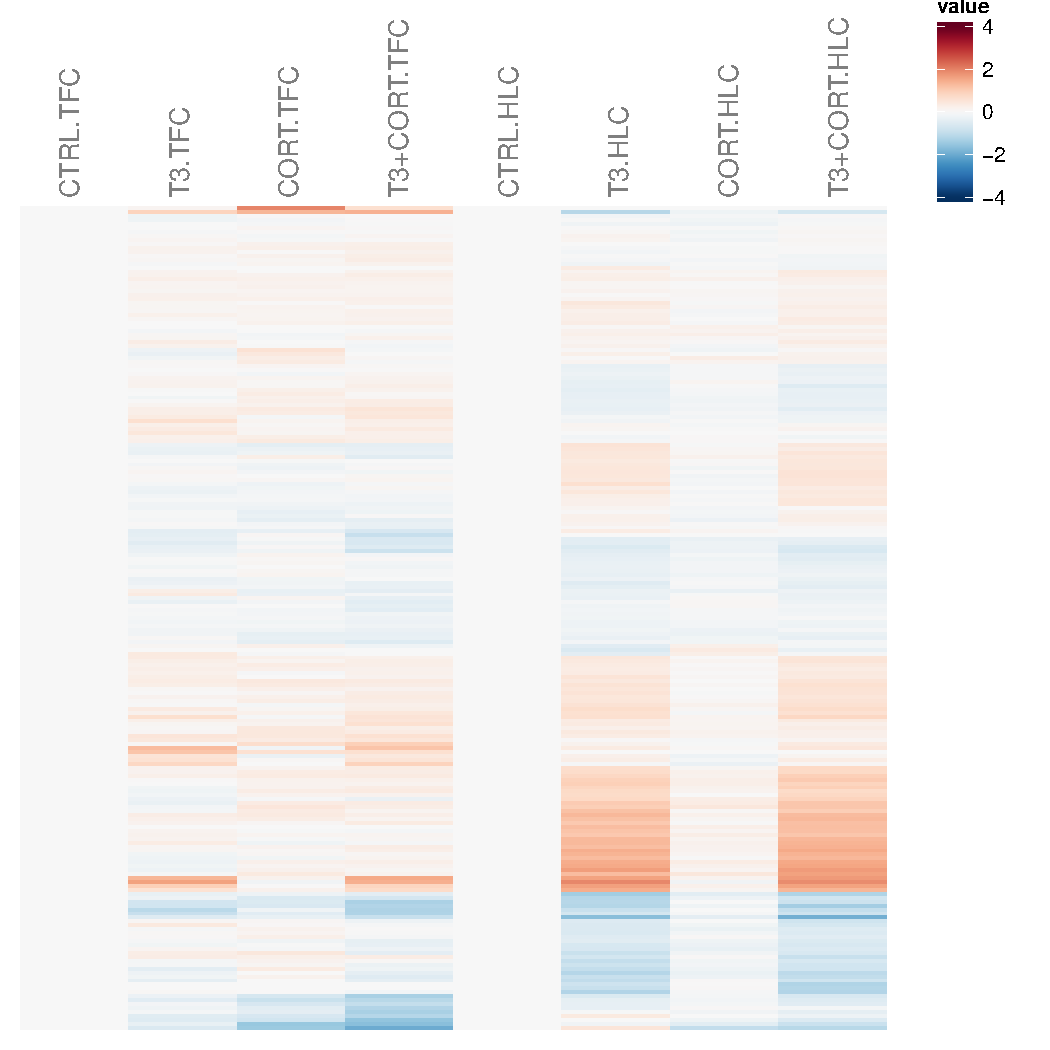
\includegraphics[width=\textwidth]
	{Figures/comparison-tfc-hlc-histones/comparison-tfc-hlc-histones-all.pdf}
	\caption{}
	\label{subfig:comparison-tfc-hlc-histones-all}
\end{subfigure}
\begin{subfigure}{0.495\textwidth}
	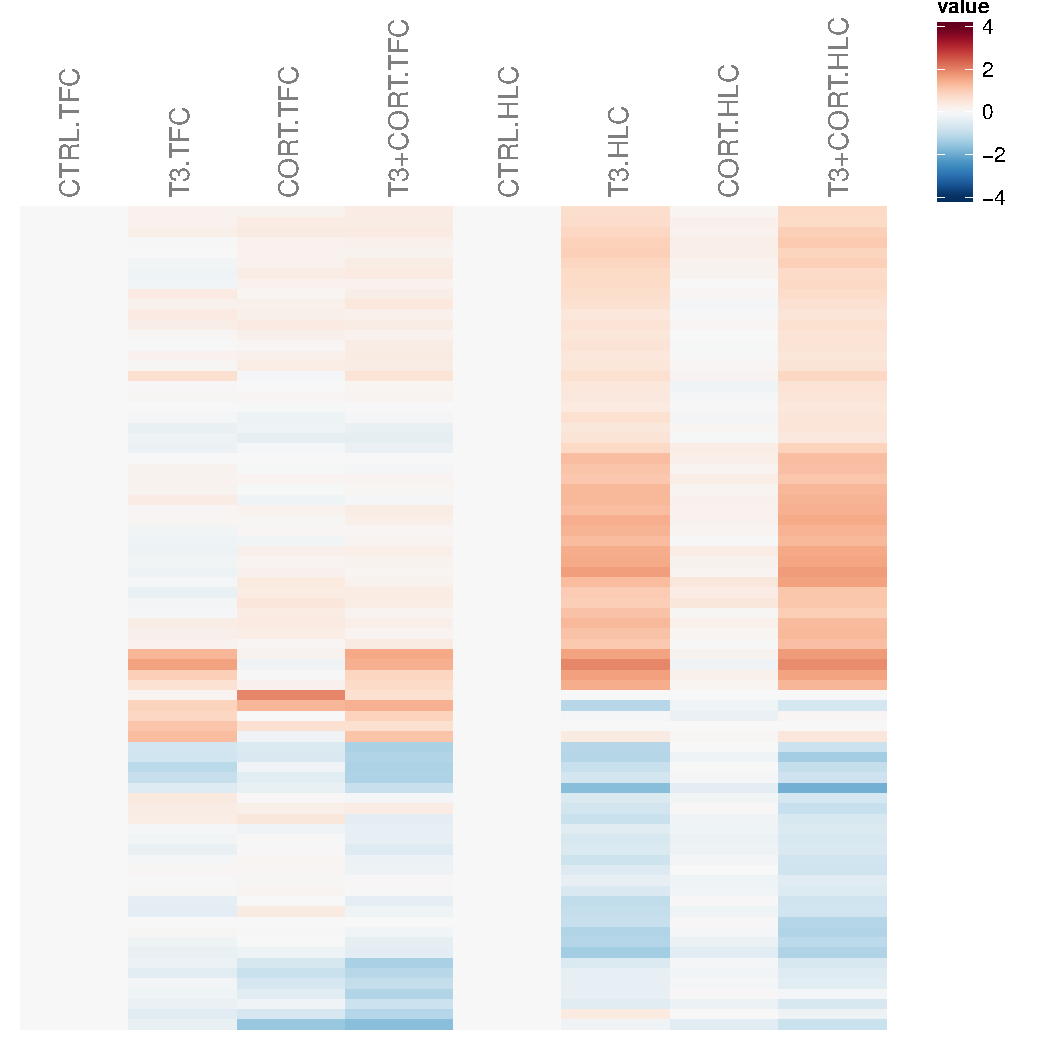
\includegraphics[width=\textwidth]
	{Figures/comparison-tfc-hlc-histones/comparison-tfc-hlc-histones-de.pdf}
	\caption{}
	\label{subfig:comparison-tfc-hlc-histones-de}
\end{subfigure}
\caption[Profils d'expression des gènes impliqués dans la modification d'histones]
{
Comparaison des profils d'expression, dans l'épiderme caudal et les bourgeons de membres postérieurs, des gènes impliqués dans les modifications post-traductionnelles d'histones.
\ref{subfig:comparison-tfc-hlc-histones-all}: Tous les gènes.
\ref{subfig:comparison-tfc-hlc-histones-de}: Sélection des gènes différentiellement exprimés dans au moins une condition.
}
\label{fig:comparison-tfc-hlc-histones}
% ===========================================================
%
% BOTTOM caption
% ------------------------
\end{figure}
% ------------------------
%
% SIDE caption
% ------------------------
%\end{SCfigure}
% ------------------------